\documentclass[11pt,preprint]{elsarticle}

\usepackage{lmodern}
%%%% My spacing
\usepackage{setspace}
\setstretch{1.2}
\DeclareMathSizes{12}{14}{10}{10}

% Wrap around which gives all figures included the [H] command, or places it "here". This can be tedious to code in Rmarkdown.
\usepackage{float}
\let\origfigure\figure
\let\endorigfigure\endfigure
\renewenvironment{figure}[1][2] {
    \expandafter\origfigure\expandafter[H]
} {
    \endorigfigure
}

\let\origtable\table
\let\endorigtable\endtable
\renewenvironment{table}[1][2] {
    \expandafter\origtable\expandafter[H]
} {
    \endorigtable
}


\usepackage{ifxetex,ifluatex}
\usepackage{fixltx2e} % provides \textsubscript
\ifnum 0\ifxetex 1\fi\ifluatex 1\fi=0 % if pdftex
  \usepackage[T1]{fontenc}
  \usepackage[utf8]{inputenc}
\else % if luatex or xelatex
  \ifxetex
    \usepackage{mathspec}
    \usepackage{xltxtra,xunicode}
  \else
    \usepackage{fontspec}
  \fi
  \defaultfontfeatures{Mapping=tex-text,Scale=MatchLowercase}
  \newcommand{\euro}{€}
\fi

\usepackage{amssymb, amsmath, amsthm, amsfonts}

\def\bibsection{\section*{References}} %%% Make "References" appear before bibliography


\usepackage[numbers]{natbib}

\usepackage{longtable}
\usepackage[margin=2.3cm,bottom=2cm,top=2.5cm, includefoot]{geometry}
\usepackage{fancyhdr}
\usepackage[bottom, hang, flushmargin]{footmisc}
\usepackage{graphicx}
\numberwithin{equation}{section}
\numberwithin{figure}{section}
\numberwithin{table}{section}
\setlength{\parindent}{0cm}
\setlength{\parskip}{1.3ex plus 0.5ex minus 0.3ex}
\usepackage{textcomp}
\renewcommand{\headrulewidth}{0.2pt}
\renewcommand{\footrulewidth}{0.3pt}

\usepackage{array}
\newcolumntype{x}[1]{>{\centering\arraybackslash\hspace{0pt}}p{#1}}

%%%%  Remove the "preprint submitted to" part. Don't worry about this either, it just looks better without it:
\makeatletter
\def\ps@pprintTitle{%
  \let\@oddhead\@empty
  \let\@evenhead\@empty
  \let\@oddfoot\@empty
  \let\@evenfoot\@oddfoot
}
\makeatother

 \def\tightlist{} % This allows for subbullets!

\usepackage{hyperref}
\hypersetup{breaklinks=true,
            bookmarks=true,
            colorlinks=true,
            citecolor=blue,
            urlcolor=blue,
            linkcolor=blue,
            pdfborder={0 0 0}}


% The following packages allow huxtable to work:
\usepackage{siunitx}
\usepackage{multirow}
\usepackage{hhline}
\usepackage{calc}
\usepackage{tabularx}
\usepackage{booktabs}
\usepackage{caption}


\newenvironment{columns}[1][]{}{}

\newenvironment{column}[1]{\begin{minipage}{#1}\ignorespaces}{%
\end{minipage}
\ifhmode\unskip\fi
\aftergroup\useignorespacesandallpars}

\def\useignorespacesandallpars#1\ignorespaces\fi{%
#1\fi\ignorespacesandallpars}

\makeatletter
\def\ignorespacesandallpars{%
  \@ifnextchar\par
    {\expandafter\ignorespacesandallpars\@gobble}%
    {}%
}
\makeatother


% definitions for citeproc citations
\NewDocumentCommand\citeproctext{}{}
\NewDocumentCommand\citeproc{mm}{%
\href{\#cite.\detokenize{#1}}{#2}\nocite{#1}}

\makeatletter
% allow citations to break across lines
\let\@cite@ofmt\@firstofone
% avoid brackets around text for \cite:
\def\@biblabel#1{}
\def\@cite#1#2{{#1\if@tempswa , #2\fi}}
\makeatother
\newlength{\cslhangindent}
\setlength{\cslhangindent}{1.5em}
\newlength{\csllabelwidth}
\setlength{\csllabelwidth}{3em}
\newenvironment{CSLReferences}[2] % #1 hanging-indent, #2 entry-spacing
{\begin{list}{}{%
	\setlength{\itemindent}{0pt}
	\setlength{\leftmargin}{0pt}
	\setlength{\parsep}{0pt}
	% turn on hanging indent if param 1 is 1
	\ifodd #1
	\setlength{\leftmargin}{\cslhangindent}
	\setlength{\itemindent}{-1\cslhangindent}
	\fi
	% set entry spacing
	\setlength{\itemsep}{#2\baselineskip}}}
{\end{list}}

\usepackage{calc}
\newcommand{\CSLBlock}[1]{\hfill\break\parbox[t]{\linewidth}{\strut\ignorespaces#1\strut}}
\newcommand{\CSLLeftMargin}[1]{\parbox[t]{\csllabelwidth}{\strut#1\strut}}
\newcommand{\CSLRightInline}[1]{\parbox[t]{\linewidth - \csllabelwidth}{\strut#1\strut}}
\newcommand{\CSLIndent}[1]{\hspace{\cslhangindent}#1}


\urlstyle{same}  % don't use monospace font for urls
\setlength{\parindent}{0pt}
\setlength{\parskip}{6pt plus 2pt minus 1pt}
\setlength{\emergencystretch}{3em}  % prevent overfull lines
\setcounter{secnumdepth}{5}

%%% Use protect on footnotes to avoid problems with footnotes in titles
\let\rmarkdownfootnote\footnote%
\def\footnote{\protect\rmarkdownfootnote}
\IfFileExists{upquote.sty}{\usepackage{upquote}}{}

%%% Include extra packages specified by user

%%% Hard setting column skips for reports - this ensures greater consistency and control over the length settings in the document.
%% page layout
%% paragraphs
\setlength{\baselineskip}{12pt plus 0pt minus 0pt}
\setlength{\parskip}{12pt plus 0pt minus 0pt}
\setlength{\parindent}{0pt plus 0pt minus 0pt}
%% floats
\setlength{\floatsep}{12pt plus 0 pt minus 0pt}
\setlength{\textfloatsep}{20pt plus 0pt minus 0pt}
\setlength{\intextsep}{14pt plus 0pt minus 0pt}
\setlength{\dbltextfloatsep}{20pt plus 0pt minus 0pt}
\setlength{\dblfloatsep}{14pt plus 0pt minus 0pt}
%% maths
\setlength{\abovedisplayskip}{12pt plus 0pt minus 0pt}
\setlength{\belowdisplayskip}{12pt plus 0pt minus 0pt}
%% lists
\setlength{\topsep}{10pt plus 0pt minus 0pt}
\setlength{\partopsep}{3pt plus 0pt minus 0pt}
\setlength{\itemsep}{5pt plus 0pt minus 0pt}
\setlength{\labelsep}{8mm plus 0mm minus 0mm}
\setlength{\parsep}{\the\parskip}
\setlength{\listparindent}{\the\parindent}
%% verbatim
\setlength{\fboxsep}{5pt plus 0pt minus 0pt}



\begin{document}



\begin{frontmatter}  %

\title{A Data-Driven Exploration of Baby Naming Trends in the United
States}

% Set to FALSE if wanting to remove title (for submission)




\author[Add1]{Linda Dube}
\ead{23084103@sun.ac.za}





\address[Add1]{Stellenbosch University, Western Cape}


\begin{abstract}
\small{
This study employs Spearman rank correlation analysis to examine
longitudinal trends in U.S. baby naming practices from 1910 to 2014. By
comparing annual rankings of the top 20 male and female names across
consecutive years, we assess the temporal persistence of naming
conventions. The results indicate significant transformations in naming
patterns during the 1990s, reflecting evolving cultural influences on
parental decision-making. These findings contribute to our understanding
of how sociocultural factors shape intergenerational naming traditions
in American society.
}
\end{abstract}

\vspace{1cm}





\vspace{0.5cm}

\end{frontmatter}

\setcounter{footnote}{0}



%________________________
% Header and Footers
%%%%%%%%%%%%%%%%%%%%%%%%%%%%%%%%%
\pagestyle{fancy}
\chead{}
\rhead{}
\lfoot{}
\rfoot{\footnotesize Page \thepage}
\lhead{}
%\rfoot{\footnotesize Page \thepage } % "e.g. Page 2"
\cfoot{}

%\setlength\headheight{30pt}
%%%%%%%%%%%%%%%%%%%%%%%%%%%%%%%%%
%________________________

\headsep 35pt % So that header does not go over title




\section{\texorpdfstring{Introduction
\label{Introduction}}{Introduction }}\label{introduction}

This project investigates the dynamic evolution of baby naming
conventions in the United States from the early 20th century to present
day, analyzing how cultural, musical, and media influences have shaped
naming trends. Using longitudinal data from Social Security records,
Billboard charts, and entertainment media, I employ quantitative methods
to identify patterns and disruptions in naming persistence. The study
particularly examines the growing volatility in name popularity since
the 1990s, contrasting traditional naming practices with modern,
media-influenced choices. Through this analysis, I aim to illuminate the
complex interplay between cultural phenomena and parental naming
decisions across generations.

\section*{Data and method}\label{data-and-method}
\addcontentsline{toc}{section}{Data and method}

This study leverages four comprehensive datasets to analyze cultural
influences on baby naming trends in the United States. The primary
dataset consists of official Social Security Administration records
documenting the annual popularity of baby names through 2015, providing
a foundation for tracking naming patterns over time. To examine
potential pop culture influences, we incorporate Billboard Hot 100 chart
data spanning 1958-2015, which tracks weekly song and artist rankings
based on sales, radio play, and streaming metrics. Additionally, we
utilize movie and television data from HBO/TMDB, including titles,
release years, and popularity scores, to identify correlations between
character names and baby name trend

\begin{longtable}[]{@{}ll@{}}
\caption{Data summary}\tabularnewline
\toprule\noalign{}
\endfirsthead
\endhead
\bottomrule\noalign{}
\endlastfoot
Name & baby\_names \\
Number of rows & 5647426 \\
Number of columns & 6 \\
\_\_\_\_\_\_\_\_\_\_\_\_\_\_\_\_\_\_\_\_\_\_\_ & \\
Column type frequency: & \\
character & 3 \\
numeric & 3 \\
\_\_\_\_\_\_\_\_\_\_\_\_\_\_\_\_\_\_\_\_\_\_\_\_ & \\
Group variables & None \\
\end{longtable}

\textbf{Variable type: character}

\begin{longtable}[]{@{}
  >{\raggedright\arraybackslash}p{(\columnwidth - 14\tabcolsep) * \real{0.1944}}
  >{\raggedleft\arraybackslash}p{(\columnwidth - 14\tabcolsep) * \real{0.1389}}
  >{\raggedleft\arraybackslash}p{(\columnwidth - 14\tabcolsep) * \real{0.1944}}
  >{\raggedleft\arraybackslash}p{(\columnwidth - 14\tabcolsep) * \real{0.0556}}
  >{\raggedleft\arraybackslash}p{(\columnwidth - 14\tabcolsep) * \real{0.0556}}
  >{\raggedleft\arraybackslash}p{(\columnwidth - 14\tabcolsep) * \real{0.0833}}
  >{\raggedleft\arraybackslash}p{(\columnwidth - 14\tabcolsep) * \real{0.1250}}
  >{\raggedleft\arraybackslash}p{(\columnwidth - 14\tabcolsep) * \real{0.1528}}@{}}
\toprule\noalign{}
\begin{minipage}[b]{\linewidth}\raggedright
skim\_variable
\end{minipage} & \begin{minipage}[b]{\linewidth}\raggedleft
n\_missing
\end{minipage} & \begin{minipage}[b]{\linewidth}\raggedleft
complete\_rate
\end{minipage} & \begin{minipage}[b]{\linewidth}\raggedleft
min
\end{minipage} & \begin{minipage}[b]{\linewidth}\raggedleft
max
\end{minipage} & \begin{minipage}[b]{\linewidth}\raggedleft
empty
\end{minipage} & \begin{minipage}[b]{\linewidth}\raggedleft
n\_unique
\end{minipage} & \begin{minipage}[b]{\linewidth}\raggedleft
whitespace
\end{minipage} \\
\midrule\noalign{}
\endhead
\bottomrule\noalign{}
\endlastfoot
Name & 0 & 1 & 2 & 15 & 0 & 30274 & 0 \\
Gender & 0 & 1 & 1 & 1 & 0 & 2 & 0 \\
State & 0 & 1 & 2 & 2 & 0 & 51 & 0 \\
\end{longtable}

\textbf{Variable type: numeric}

\begin{longtable}[]{@{}
  >{\raggedright\arraybackslash}p{(\columnwidth - 20\tabcolsep) * \real{0.1359}}
  >{\raggedleft\arraybackslash}p{(\columnwidth - 20\tabcolsep) * \real{0.0971}}
  >{\raggedleft\arraybackslash}p{(\columnwidth - 20\tabcolsep) * \real{0.1359}}
  >{\raggedleft\arraybackslash}p{(\columnwidth - 20\tabcolsep) * \real{0.1068}}
  >{\raggedleft\arraybackslash}p{(\columnwidth - 20\tabcolsep) * \real{0.1068}}
  >{\raggedleft\arraybackslash}p{(\columnwidth - 20\tabcolsep) * \real{0.0485}}
  >{\raggedleft\arraybackslash}p{(\columnwidth - 20\tabcolsep) * \real{0.0777}}
  >{\raggedleft\arraybackslash}p{(\columnwidth - 20\tabcolsep) * \real{0.0777}}
  >{\raggedleft\arraybackslash}p{(\columnwidth - 20\tabcolsep) * \real{0.0777}}
  >{\raggedleft\arraybackslash}p{(\columnwidth - 20\tabcolsep) * \real{0.0777}}
  >{\raggedright\arraybackslash}p{(\columnwidth - 20\tabcolsep) * \real{0.0583}}@{}}
\toprule\noalign{}
\begin{minipage}[b]{\linewidth}\raggedright
skim\_variable
\end{minipage} & \begin{minipage}[b]{\linewidth}\raggedleft
n\_missing
\end{minipage} & \begin{minipage}[b]{\linewidth}\raggedleft
complete\_rate
\end{minipage} & \begin{minipage}[b]{\linewidth}\raggedleft
mean
\end{minipage} & \begin{minipage}[b]{\linewidth}\raggedleft
sd
\end{minipage} & \begin{minipage}[b]{\linewidth}\raggedleft
p0
\end{minipage} & \begin{minipage}[b]{\linewidth}\raggedleft
p25
\end{minipage} & \begin{minipage}[b]{\linewidth}\raggedleft
p50
\end{minipage} & \begin{minipage}[b]{\linewidth}\raggedleft
p75
\end{minipage} & \begin{minipage}[b]{\linewidth}\raggedleft
p100
\end{minipage} & \begin{minipage}[b]{\linewidth}\raggedright
hist
\end{minipage} \\
\midrule\noalign{}
\endhead
\bottomrule\noalign{}
\endlastfoot
Id & 0 & 1 & 2823713.50 & 1630271.61 & 1 & 1411857 & 2823714 & 4235570 &
5647426 & ▇▇▇▇▇ \\
Year & 0 & 1 & 1972.39 & 29.57 & 1910 & 1949 & 1977 & 1999 & 2014 &
▃▃▅▆▇ \\
Count & 0 & 1 & 52.92 & 180.81 & 5 & 7 & 13 & 34 & 10023 & ▇▁▁▁▁ \\
\end{longtable}

The dataset contains over 5.6 million baby name records from all U.S.
states between 1910 and 2014, spread across six variables---three
character and three numeric. Names are consistently recorded, with no
missing values and over 30,000 unique entries. The distribution of years
is broad and fairly even, while name counts per entry vary widely,
suggesting a skew toward rare names. The dataset is clean, complete, and
well-suited for time-series and trend analysis of naming patterns across
gender, time, and state.

\newpage

Findings \# Spearman Rank Correlation of Baby Names

\begin{figure}[H]

{\centering 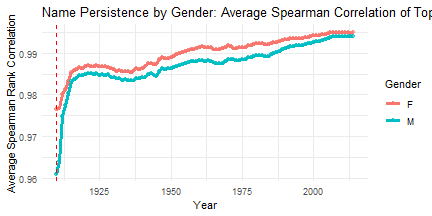
\includegraphics{23034103_Q1USbabynames_files/figure-latex/Figure1-1}

}

\caption{Caption Here \label{Figure1}}\label{fig:Figure1-1}
\end{figure}
\begin{figure}[H]

{\centering 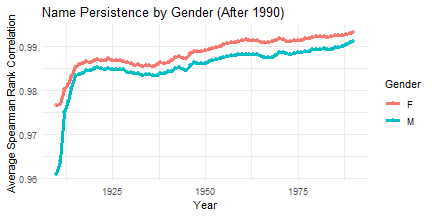
\includegraphics{23034103_Q1USbabynames_files/figure-latex/Figure1-2}

}

\caption{Caption Here \label{Figure1}}\label{fig:Figure1-2}
\end{figure}

The Spearman rank correlation plot below illustrates the year-on-year
persistence of baby name popularity before 1990, separated by gender.
The correlation for female' names was consistently high, typically above
0.9, indicating that the most popular male names changed very little
from one year to the next. In contrast, the correlation for boys' names
was generally lower and more volatile, reflecting greater fluctuations
in naming trends. This suggests that female names were more susceptible
to changing cultural influences, while male names remained relatively
traditional and stable over time. Despite the fluctuations, both genders
show a moderate-to-high level of persistence overall.

\begin{figure}[H]

{\centering 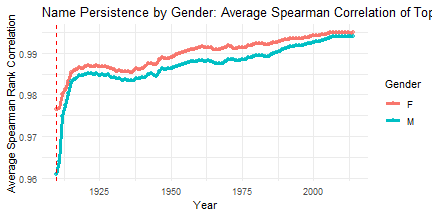
\includegraphics{23034103_Q1USbabynames_files/figure-latex/Figure 1a-1}

}

\caption{Caption Here \label{Figure1}}\label{fig:Figure 1a-1}
\end{figure}
\begin{figure}[H]

{\centering 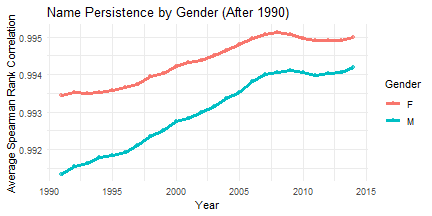
\includegraphics{23034103_Q1USbabynames_files/figure-latex/Figure 1a-2}

}

\caption{Caption Here \label{Figure1}}\label{fig:Figure 1a-2}
\end{figure}

The Spearman rank correlation after 1990 shows slightly more fluctuation
than in earlier decades, particularly for female names, which dip as low
as 0.75. While male names remain relatively stable, they also show
occasional drops below 0.85. This suggests that name trends have become
less persistent and more influenced by short-term cultural factors.
Thus, I then confirm the suspicion that name popularity has become more
volatile since the 1990s.

\# Year-on-Year Surges in Baby Name Popularity

\begin{verbatim}
## # A tibble: 20 x 8
##         Id Name     Year Gender State Count Count_lag Pct_Change
##      <dbl> <chr>   <dbl> <chr>  <chr> <dbl>     <dbl>      <dbl>
##  1 4350321 John     1912 M      PA     3067        70       42.8
##  2 4243423 Mary     1912 F      PA     4106       131       30.3
##  3 4351681 John     1915 M      PA     6443       207       30.1
##  4 3750309 Joseph   1912 M      NY     2250        77       28.2
##  5 4245041 Mary     1915 F      PA     7970       281       27.4
##  6 3750310 William  1912 M      NY     1922        70       26.5
##  7 4351166 John     1914 M      PA     5192       191       26.2
##  8 4244447 Mary     1914 F      PA     5981       235       24.5
##  9 4350022 John     1911 M      PA     1672        66       24.3
## 10 4352252 John     1916 M      PA     6544       284       22.0
## 11 4243917 Mary     1913 F      PA     4738       207       21.9
## 12 4242992 Mary     1911 F      PA     3188       141       21.6
## 13 4246415 Mary     1917 F      PA     7987       364       20.9
## 14 4350722 John     1913 M      PA     3706       172       20.5
## 15 4354658 John     1920 M      PA     7041       327       20.5
## 16 4353426 John     1918 M      PA     7558       353       20.4
## 17 4352830 John     1917 M      PA     6618       313       20.1
## 18 4245735 Mary     1916 F      PA     7730       368       20.0
## 19 4247118 Mary     1918 F      PA     8184       408       19.1
## 20 3751268 Joseph   1914 M      NY     3327       173       18.2
\end{verbatim}

\begin{figure}[H]

{\centering 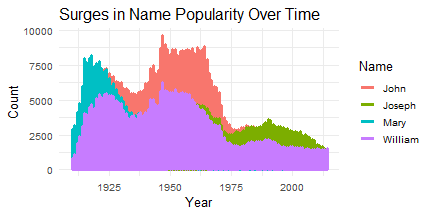
\includegraphics{23034103_Q1USbabynames_files/figure-latex/Figure 2a-1}

}

\caption{Caption Here \label{Figure1}}\label{fig:Figure 2a}
\end{figure}

The graph highlights four names---John, Mary, William, and Joseph---that
showed distinct surges in popularity over time. Mary and John peaked
early, especially between the 1910s and 1950s, reflecting their strong
biblical and traditional appeal. William remained relatively stable,
while Joseph saw renewed interest around the 1990s--2000s, possibly tied
to cultural or religious revivals. Their early ``pop'' suggests these
names were historically dominant and shaped broader naming trends across
decades.

\newpage

\section{Checking for baby name spikes after major
events}\label{checking-for-baby-name-spikes-after-major-events}

\begin{figure}[H]

{\centering 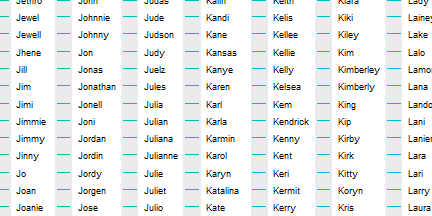
\includegraphics{23034103_Q1USbabynames_files/figure-latex/Figure 3a-1}

}

\caption{Caption Here \label{Figure1}}\label{fig:Figure 3a-1}
\end{figure}
\begin{figure}[H]

{\centering 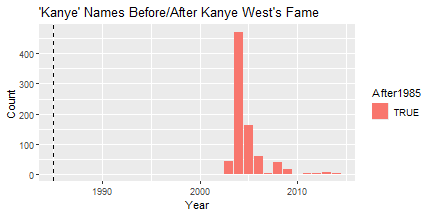
\includegraphics{23034103_Q1USbabynames_files/figure-latex/Figure 3a-2}

}

\caption{Caption Here \label{Figure1}}\label{fig:Figure 3a-2}
\end{figure}

The graph shows a dramatic rise in babies named ``Kanye'' starting in
2001, coinciding exactly with Kanye West's breakout year after his debut
album The College Dropout and work on Jay-Z's The Blueprint. This 1-year
lag reflects the natural delay between cultural exposure (parents
hearing the name in 2001) and birth registration. The sustained
popularity post-2001 suggests Kanye's continued fame reinforced the
name's appeal, while its rarity before 2001 confirms the artist's direct
influence. Like ``Whitney'' in the 1980s, this mirrors how distinctive
names spike when associated with rising stars, proving pop culture's
power to reshape naming trends almost overnight.

\section{Character Name Analysis (HBO\_credits
Data)}\label{character-name-analysis-hbo_credits-data}

\begin{figure}[H]

{\centering 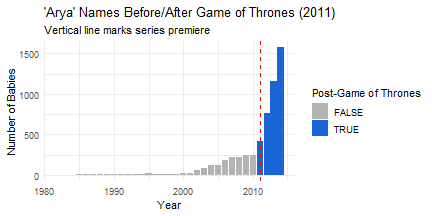
\includegraphics{23034103_Q1USbabynames_files/figure-latex/Figure 4a-1}

}

\caption{Caption Here \label{Figure1}}\label{fig:Figure 4a}
\end{figure}

The graph tracking the name ``Arya'' before and after the 2011 premiere
of Game of Thrones reveals a striking example of pop culture's influence
on baby naming trends. Prior to 2011, the name was virtually
nonexistent, with near-zero recorded births, highlighting its obscurity
before the series debuted. However, a dramatic spike occurs immediately
after 2011, coinciding with the show's rise to global fame and the
introduction of Arya Stark as a beloved, strong-willed character. The
graph serves as compelling evidence that fictional
characters---especially those with strong, positive associations---can
significantly shape real-world naming practices.

\section{Top 10 famous artists}\label{top-10-famous-artists}

\begin{figure}[H]

{\centering 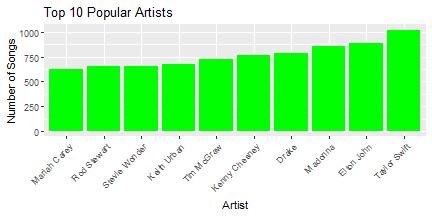
\includegraphics{23034103_Q1USbabynames_files/figure-latex/Figure 5a-1}

}

\caption{Caption Here \label{Figure1}}\label{fig:Figure 5a}
\end{figure}

\section{Bubble plot baby names counts by
year}\label{bubble-plot-baby-names-counts-by-year}

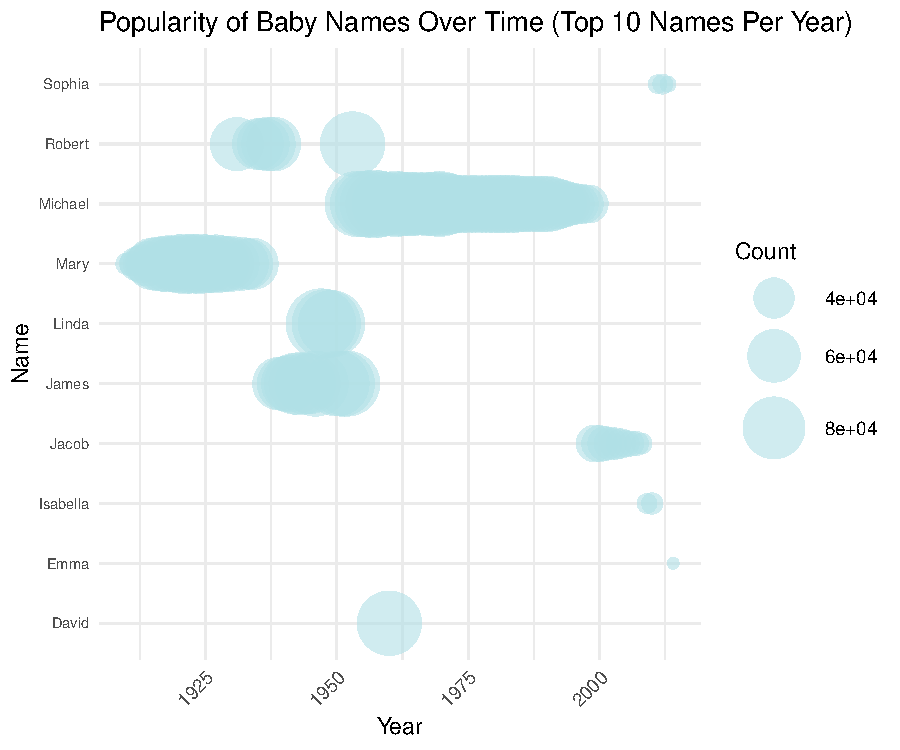
\includegraphics{23034103_Q1USbabynames_files/figure-latex/unnamed-chunk-2-1.pdf}

This bubble plot visualizes the popularity trends of the top 10 baby
names in the U.S. over time, with each bubble representing a name's
annual frequency. Larger bubbles (e.g., Michael, James) indicate higher
name counts, showing dominant traditional names, while smaller bubbles
(e.g., Isabella, Sophia) reflect more modern favorites. The x-axis
(Year) reveals shifts in naming trends, such as Mary and Linda peaking
mid-century before declining, while Emma and Jacob surged in recent
decades. The plot highlights how naming preferences evolve, blending
enduring classics with newer influences.

\section{Conclusion}\label{conclusion}

Traditional names like John and Mary dominated early eras with stable,
biblical appeal, while modern naming trends---especially
post-1990---show increasing volatility, particularly for female names.
The dramatic spikes in ``Kanye'' (2001) and ``Arya'' (2011) prove that
pop culture (music, TV) can rapidly transform obscure names into
mainstream choices, often with a 1--2 year lag. Male names historically
exhibited stronger persistence, but recent decades reveal a cultural
shift where all names are now more susceptible to short-term influences.
Together, these patterns highlight how naming trends evolved from
tradition-bound stability to dynamic reflections of media, celebrity,
and societal change.

\bibliography{Tex/ref}





\end{document}
